\documentclass{article}
\usepackage{iclr2026_conference,times}

\input{math_commands.tex}

\usepackage[colorlinks=true,linkcolor=black!70!blue,citecolor=black!70!blue,urlcolor=black!70!blue]{hyperref}
\usepackage{url}
\usepackage{graphicx}
\usepackage{booktabs}
\usepackage{xcolor}
\usepackage{enumitem}
\usepackage{amsmath,amssymb,amsfonts,amsthm}
\usepackage{microtype}

% Draft markers. Every marker names the evidence needed to remove it.
\definecolor{tbdcol}{HTML}{C0561B}
\newcommand{\tbd}[1]{{\color{tbdcol}\textbf{TBD}~#1}}
\newcommand{\sieve}{\textsc{Sieve}}
\newcommand{\gplus}{G_{+}}

% Theorem-like environments used by appendix.tex.
\theoremstyle{definition}
\newtheorem{definition}{Definition}[section]
\newtheorem{theorem}{Theorem}[section]
\newtheorem{remark}{Remark}[section]

\title{When Does Joint Key-Cache Allocation Pay?\\
Context-Dependent Regimes in Quantization and Eviction}

\author{Anonymous authors \\ Paper under double-blind review}

% \iclrfinalcopy
\begin{document}

\maketitle

\begin{abstract}
KV-cache compressors can spend a memory budget by quantizing every token, evicting tokens, or mixing both actions.  Existing work shows how to build such hybrids; we ask when the mixed interior improves over its two endpoints.  Under a separable local surrogate for attention-output distortion, key-token precision is a discrete rate-allocation problem that includes a normalized zero-rate cost.  A finite-bit tier is dominated when its absolute logit-noise cost exceeds that zero-rate cost, yielding a measurable tier-extinction coordinate.  Across six LLMs and 25 model--context cells spanning 4k--256k, with allocations evaluated by exact attention-output recomputation, this coordinate orders the mixed allocator's advantage under a symmetric lagged-information comparison (Spearman $\rho=-0.978$, $-0.915$ after accounting for model identity).  The crossing is architecture-conditioned rather than universal, and increasing context moves fixed models toward an eviction-like corner.  Measurements over 4,096 decode tokens further reveal two output-error timescales: the head-level family label remains stable (p90 regret $1.00$ in six cells), while a frozen token allocation costs $2.52$--$4.30\times$ a one-step-old allocation.  A completed end-task campaign does not validate the regime map as an accuracy router: uniform quantization is the strongest fixed policy in 34/36 valid cells, and the calibrated router has 17 clear losses.  Thus the map characterizes local distortion regimes rather than establishing downstream effectiveness.
\end{abstract}

% ===========================================================================
\section{Introduction}
% ===========================================================================

At long context, the KV cache can bound batch size and decode throughput.  A cache budget admits at least three actions: assign every token one low precision~\citep{liu2024kivi,hooper2024kvquant,zandieh2025turboquant}, retain selected tokens at a higher precision~\citep{zhang2023h2o,liu2023scissorhands,li2024snapkv,xiao2024streamingllm}, or mix zero and finite rates across tokens.  The last option is no longer hypothetical: DiffKV and HqeKV combine pruning with multiple precision levels~\citep{zhang2025diffkv,wang-etal-2026-hqekv}.  What remains unclear is whether the extra interior choices are useful for a given model and deployment context, or whether a simpler endpoint already suffices.

We study that missing question.  The motivating reversal is within one model, not between leaderboards: from 8k to 128k, Llama-3.3-70B's dead-2-bit fraction rises from $5.5\%$ to $41.4\%$, its hindsight portfolio gain falls from $3.17\times$ to $1.40\times$, and the share of heads where the interior beats both endpoints by $2\times$ falls from $87.4\%$ to $21.3\%$.  A verdict at one context therefore need not transfer to another.

Our lens is a joint key-token action space.  We derive a first-order, separable attention-output surrogate for finite-bit key noise; we place eviction at zero rate using an explicitly stated local approximation; and we solve the actual discrete allocation over hardware tiers.  This view exposes two different boundaries.  Insufficient variation in token importance removes the benefit of unequal precision, while excessive absolute noise makes low-bit tiers worse than zero rate.  We call the resulting picture an \emph{architecture-conditioned regime map}; the present data establish its mixed-to-eviction side most strongly.

\begin{figure}[t]
  \centering
  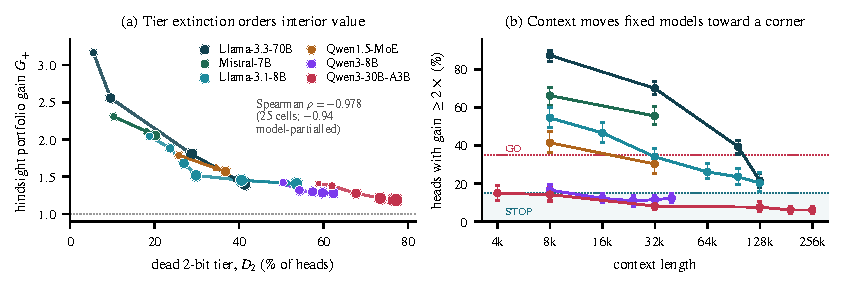
\includegraphics[width=\linewidth]{figures/fig1_regime.pdf}
  \vspace{-4mm}
  \caption{\textbf{Measured symmetric results.} Both the mixed allocator and the eviction endpoint use lagged information; exact recomputation scores both. \textbf{(a)} The tier-extinction coordinate $D_2$ strongly orders the primary continuous response, hindsight portfolio gain $\gplus$. Arrows show increasing context. \textbf{(b)} The secondary $2\times$ band statistic shows that context moves fixed models across predeclared output-error bands. Error bars are 90\% layer-cluster intervals. The 25-cell extension spans 4k--256k; thresholds are not universal across architectures.}
  \label{fig:regime}
  \vspace{-3mm}
\end{figure}

Our contributions are:
\begin{enumerate}[leftmargin=*,itemsep=1pt,topsep=2pt]
  \item \textbf{A common action space and a regime question.} We formulate within-head key-token precision and eviction under one local output-distortion surrogate, distinguish the exact set-eviction error from the separable zero-rate approximation, and ask when the discrete interior beats both endpoints.
  \item \textbf{An architecture-conditioned regime indicator.} Across 25 cells, the dead-tier fraction strongly orders the interior's measured attention-output advantage, including under symmetric lagged information and model-controlled analyses; the critical value remains architecture-specific.
  \item \textbf{Context traversal and two refresh timescales.} Context changes tier viability within a fixed model.  The output-error-optimal family label changes slowly, whereas token allocations go stale quickly; GQA grouping and a key-only score cascade quantify the costs of a future controller.
\end{enumerate}

Concurrent RDKV also derives joint eviction--quantization rate allocation~\citep{zhang2026rdkv}.  Our paper-specific contribution is complementary: measuring and ordering \emph{when} a nontrivial token-precision interior lowers attention-output error and how that answer changes with context.  Section~\ref{sec:related} gives a precise comparison to RDKV and other allocation axes.

% ===========================================================================
\section{Joint token-rate allocation as a common foundation}
\label{sec:framework}
% ===========================================================================

\paragraph{Scope and local quantization surrogate.}
For one query $q$, keys $k_i$, and values $v_i$, let
$s_i=q^\top k_i/\sqrt d$, $a=\operatorname{softmax}(s)$, and
$o=\sum_i a_i v_i$.  Quantizing key $i$ perturbs its logit by $\delta_i$.
The first-order output change is
\begin{equation}
  \Delta o \approx \sum_i a_i(v_i-o)\delta_i .
  \label{eq:linear}
\end{equation}
If residual perturbations are zero mean and cross-token covariance terms vanish,
\begin{equation}
  \mathbb E\|\Delta o\|^2
  \approx \sum_i w_i d_{b_i}, \qquad
  w_i=a_i^2\|v_i-o\|^2,\quad d_b=\operatorname{Var}(\delta_b).
  \label{eq:surrogate}
\end{equation}
Only a common-mode logit shift is canceled exactly by softmax; arbitrary token-dependent bias and covariance are outside this surrogate.  We therefore use Eq.~\ref{eq:surrogate} to \emph{choose} allocations, never to score their reported error.

\paragraph{Exact eviction versus a zero-rate surrogate.}
For an evicted set $E$, define $A_E=\sum_{i\in E}a_i$.  Renormalizing the surviving attention gives the exact identity
\begin{equation}
 o_{\setminus E}-o
 =-\frac{\sum_{i\in E}a_i(v_i-o)}{1-A_E},\qquad
 \|o_{\setminus E}-o\|^2
 =\frac{\left\|\sum_{i\in E}a_i(v_i-o)\right\|^2}{(1-A_E)^2}.
 \label{eq:exact-eviction}
\end{equation}
The denominator and cross-token inner products make set eviction nonseparable.  For a singleton $j$, the exact error magnitude is
$a_j\|v_j-o\|/(1-a_j)$, as derived by CAOTE~\citep{goel2025caote}.
To include zero rate in a token-separable allocator, we use the small-evicted-mass, cross-term-free approximation
$\widetilde D_0(E)=\sum_{i\in E}w_i$ and normalize its \emph{absolute} cost to $d_0=1$.  Eviction is therefore a zero-rate action \emph{inside the surrogate}, not an exact independent-token equality.

\paragraph{The implemented discrete allocation.}
For available integer tiers $\mathcal B=\{0,1,2,3,4,5,6,8\}$ and an average key budget $B$, we solve
\begin{equation}
 \min_{b_i\in\mathcal B}\sum_i w_i d_{b_i}
 \quad\text{s.t.}\quad \sum_i b_i\le BL,
 \qquad
 b_i^\star(\lambda)=\arg\min_{b\in\mathcal B}\{w_i d_b+\lambda b\}.
 \label{eq:discrete}
\end{equation}
A bisection on $\lambda$ enforces the budget.  If bits are relaxed to be continuous and $d_b\propto4^{-b}$, the stationary rule becomes
\begin{equation}
 b_i^\star=\log_2a_i+\log_2\|v_i-o\|+c .
 \label{eq:continuous}
\end{equation}
Equation~\ref{eq:continuous} explains the reverse-water-filling shape, but Eq.~\ref{eq:discrete} is the optimizer used in experiments.  Adding the value factor changes our aggregate ladder-width statistic by at most $0.035$ bits in the measured configurations; this is not a per-token bound and does not replace a direct allocation ablation.

\paragraph{Two coordinates, not one universal phase boundary.}
If $d_b\ge d_0$, tier $b$ consumes bits without lowering the surrogate cost and is therefore dominated.  This condition is sufficient for extinction; $d_b<d_0$ is not sufficient for membership in the lower convex envelope.  We summarize the sharp side by
\begin{equation}
 D_2=H^{-1}\sum_{h=1}^{H}\mathbb I[d_{h,2}\ge d_0],
 \label{eq:d2}
\end{equation}
the fraction of heads in a model--context cell whose 2-bit tier is dominated.  The diffuse side is different: unequal allocation has little leverage when the spread of token importance is narrower than the tier spacing.  For attention-only importance,
$\operatorname{std}_i(\log_2a_i)=\tau/\ln2$ is an algebraic identity, not evidence of optimality.  Thus $D_2$ primarily measures approach to the eviction-like corner; a dispersion coordinate is also required to establish the uniform corner.  Finally, $D_2$ contains no explicit $L$, but it is measured \emph{at} a context and changes with context.

% ===========================================================================
\section{Measurement protocol}
\label{sec:protocol}
% ===========================================================================

\paragraph{Models, contexts, and statistical units.}
We evaluate Llama-3.1-8B and Llama-3.3-70B~\citep{grattafiori2024llama3}, Mistral-7B~\citep{jiang2023mistral}, Qwen1.5-MoE-A2.7B~\citep{qwen2024moe}, Qwen3-8B, and Qwen3-30B-A3B~\citep{yang2025qwen3}.  The strict symmetric R3 grid has 16 model--context cells between 8k and 128k and 29,312 query-head--configuration aggregates.  Boundary extension R6 has 25 cells spanning 4k--256k and 44,416 such aggregates.  Across the six architectures there are 10,240 query-head positions and 2,016 KV-head positions counted once; contexts reuse those heads.  Statistical claims therefore treat models/cells, not raw heads, as independent units.  PG-19 text~\citep{rae2020pg19} supplies the haystack, and every retrieval cell passes a full-cache needle-retrieval gate.

\paragraph{Compression and budget.}
Keys are quantized with TurboQuant$_{\rm mse}$~\citep{zandieh2025turboquant}, using random rotation and Lloyd--Max scalar quantization~\citep{lloyd1982least}.  The headline budget is $B=3$ \emph{key bits per context token}; tier 0 evicts and tier 8 stores an 8-bit key.  Values remain uncompressed, and the accounting excludes scale, index, metadata, protected-window, and packing costs.  It is therefore a matched key-bit experiment, not a matched total-KV-byte system comparison.

\paragraph{Information contract and endpoints.}
The primary R3/R6 comparison is symmetric: both the mixed allocator and eviction endpoint use only lagged attention information, while positions unseen by that score remain at the maximum tier.  The endpoints are uniform 3-bit key quantization and accumulated-attention eviction retaining the number of 8-bit keys allowed by the same key-bit budget.  The headline corner set is named \emph{uniform+accum}; a robustness analysis takes the minimum error over five available corners.  Oracle/current-query results are retained only as upper bounds.  The original allocation is per query head; the co-design study separately enforces one allocation per shared KV head.

\paragraph{Exact response and metrics.}
For every assignment we quantize the real keys, recompute attention, and measure the resulting output error exactly.  For head $h$,
\begin{equation}
 g_h=\frac{\min(D_h^{\rm uniform},D_h^{\rm evict})}{D_h^{\rm mixed}},
 \qquad
 \gplus=\exp\!\left[H^{-1}\sum_h\log\max(g_h,1)\right].
 \label{eq:metrics}
\end{equation}
$\gplus$ is the primary continuous cell response.  It is a retrospective, hindsight portfolio statistic, not achieved router performance.  The share of heads with $g_h\ge2$ (the ``band'') is a secondary operational summary.  Correlations are reported over cells, with model-partialled and model-resampled checks where available.

% ===========================================================================
\section{When does the interior pay?}
\label{sec:results}
% ===========================================================================

\paragraph{The advantage survives a fair information comparison.}
In the 16-cell R3 grid, demoting both the mixed allocator and eviction endpoint to lagged information retains roughly half of the apparent asymmetric advantage.  The symmetric band remains $1.2$--$12.5$ points above the all-oracle band in all 16 cells, but five cells are now STOP (band $<15\%$) and five are NARROW ($15$--$35\%$).  The continuous hindsight portfolio gain ranges from $1.05\times$ to $3.21\times$.  Most importantly for the regime claim, $D_2$ still orders the symmetric band at $\rho=-0.985$.  Figure~\ref{fig:evidence}a exposes all three information contracts rather than labeling the asymmetric E2 result as symmetric.

\begin{figure}[t]
  \centering
  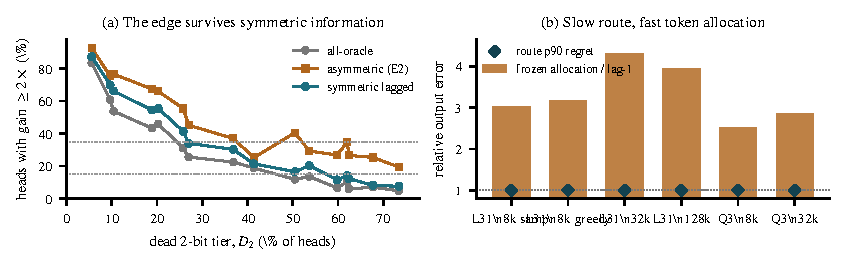
\includegraphics[width=\linewidth]{figures/fig2_evidence.pdf}
  \vspace{-4mm}
  \caption{\textbf{Measured robustness and timing.} \textbf{(a)} On the same 16 cells, the honest lagged-versus-lagged advantage is smaller than the asymmetric E2 estimate but remains ordered by $D_2$. The band is secondary and depends on the named corner set. \textbf{(b)} In six R5 cells, retaining the calibration-time \emph{policy choice} has p90 regret $1.00$ through 4,096 generated tokens, whereas freezing the token assignment costs $2.52$--$4.30\times$ a one-step-old assignment at the valid horizon.}
  \label{fig:evidence}
  \vspace{-3mm}
\end{figure}

\paragraph{Tier extinction orders value, but the crossing is model-conditioned.}
Extending to 25 cells, $D_2$ has Spearman $\rho=-0.978$ with both $\gplus$ and the band; residualizing model identity leaves $\rho=-0.915$.  A log-linear fit has leave-one-model-out error of $2.60$ band points.  Pooled monotone crossings occur near $D_2=29.0\%$ (GO) and $54.1\%$ (STOP), but they are not universal thresholds: Llama-3.1-8B remains at $20.2\%$ band at $D_2=53.7\%$, while Qwen3-8B is at $12.2\%$ band at $D_2=54.3\%$.  This eight-point disagreement across $0.6$ points of $D_2$ exceeds prompt uncertainty and identifies architecture scatter.  We therefore use $D_2$ as an ordering coordinate and fit any operational boundary per architecture.

The band also saturates near zero and can exhibit noise-level inversions, whereas $\gplus$ remains monotone along the measured Qwen3-8B trajectory.  This is why Fig.~\ref{fig:regime}a and our claims lead with the continuous response.  Prompt-block standard deviation is $0.4$--$3.0$ band points, while replacing the accumulated-attention corner with the five-corner minimum shifts the band by $-5.1$ to $-8.6$ points and can change a verdict.  Every band number must therefore name its information and corner sets.

\tbd{[R10: predictor comparison] Compare $D_2$ prospectively with RateQuant's AM/GM or $\operatorname{var}(\log w)$ heterogeneity, entropy/Gini, and context-only baselines under a fixed leave-model-out protocol.}

\paragraph{Context traverses the map.}
Every measured model trajectory moves generally toward larger tier extinction with context, though no single global boundary fits all architectures.  Llama-3.3-70B moves from GO at 8k to NARROW at 128k; Qwen3-8B moves from NARROW at 8k to STOP by 16k under the uniform+accum corner.  The mechanism is mostly an absolute-length effect: $\tau$ is generally convex in $\log L$.  Reaching the trained/RoPE cap adds a real residual of about $+0.21$ in Qwen3-8B and Qwen3-30B, but no comparable excess in Llama-3.1-8B and none at $0.75$ of the cap.  Context and architecture therefore both matter; the data do not support a universal RoPE-triggered transition.

\paragraph{The surrogate is useful, not exact.}
Across the original configuration grid, the median ratio between surrogate-predicted and exactly recomputed gain lies in $[0.79,1.34]$.  Because tier costs and evaluation data are not yet fully disjoint, we treat this as model-fit validation rather than held-out prediction.  Exact recomputation protects the empirical ordering from the approximation, but it does not validate every term of Eq.~\ref{eq:surrogate}.

\tbd{[A-VALUE] Run a direct value-aware versus attention-only allocation ablation, reporting tier-assignment changes and exact output error; the current $0.035$-bit result concerns only an aggregate width statistic.}

% ===========================================================================
\section{Deployment implications and limits}
\label{sec:deployment}
% ===========================================================================

The completed co-design experiments expose two refresh timescales in attention-output error.  A head's output-error-optimal family label was stable over 4,096 generated tokens in six measured cells, while token assignments inside a mixed head required a short refresh schedule (Fig.~\ref{fig:evidence}b).  This stability does not establish an end-task router.  The relevant measured costs are:

\begin{table}[t]
\centering
\small
\setlength{\tabcolsep}{4pt}
\caption{Completed deployment-facing measurements. These are output-error results, not end-task or throughput claims.}
\label{tab:deployment}
\begin{tabular}{@{}p{0.29\linewidth}p{0.22\linewidth}p{0.41\linewidth}@{}}
\toprule
\textbf{Constraint} & \textbf{Measurement} & \textbf{Implication} \\
\midrule
Family label over 4,096 tokens & p90 output-error regret $1.00$ in 6/6 cells & Temporally stable in these measured cells \\
Frozen token assignment & $2.52$--$4.30\times$ lag-1 error & Re-budget mixed heads quickly \\
Shared GQA allocation & $1.000/1.136/1.316\times$ at $n_{\rm rep}=1/4/8$ & Route per KV head, with a measured discount \\
4-bit current-query cascade & closes $82$--$91\%$ (median $89\%$) of lag penalty & Recover scores from base-tier keys \\
\bottomrule
\end{tabular}
\vspace{-2mm}
\end{table}

These facts motivated the tested \sieve{} selector: estimate the regime at a deployment context, choose a uniform, mixed, or eviction-like policy per KV head, and refresh mixed-head assignments from a 4-bit base pass.  Under the completed end-task contract, however, the calibrated selector is not a safe general policy.  The design remains an output-error hypothesis rather than an achieved end-task method.

\paragraph{End-task transfer.}
The completed R8 campaign does not validate the output-error map as an accuracy router.  Uniform quantization is the strongest fixed arm in 34/36 valid task--budget cells; the calibrated router has 17 clear losses, all on Llama, and the phase-band/accuracy-gain Spearman correlation is $-0.70$, opposite the prespecified direction.  The new sparse baselines improve on SnapKV but do not reverse uniform's broad advantage.  On two natural forced-choice development blocks, the label-seeing candidate oracle adds only $3/52$ over the best fixed Llama policy and a descriptive $2/52$ for Qwen; the Qwen protocol formally stops first because FP accuracy is $24/52<0.50$.  Both proxy outcomes are suppressed by sequential gates, and confirmation remains unopened.

\tbd{[SYSTEM] Measure nested-tier storage, scale/index/metadata bytes, protected-window cost, and packed-kernel latency/throughput. The current experiment establishes key-bit output error, not total-KV memory or speedup.}

% ===========================================================================
\section{Related and concurrent work}
\label{sec:related}
% ===========================================================================

\paragraph{Quantization, eviction, and hybrid token storage.}
KV quantizers use per-channel/per-token integer schemes~\citep{liu2024kivi,hooper2024kvquant}, rotations or sketches~\citep{zandieh2025turboquant,zandieh2024qjl}, and salient-token mixed precision~\citep{yang2024mikv,he2024zipcache}.  Evictors use accumulated or windowed attention~\citep{zhang2023h2o,li2024snapkv,liu2023scissorhands,xiao2024streamingllm} and allocate keep budgets across layers or heads~\citep{cai2024pyramidkv,feng2024adakv}.  The historical split is not strict: archival DiffKV routes tokens among high precision, low precision, and pruning and supplies an on-GPU manager~\citep{zhang2025diffkv}; HqeKV optimizes among full precision, several quantized levels, and eviction using joint K--V importance~\citep{wang-etal-2026-hqekv}.  Our novelty is not hybrid tiering.  We derive and test when an intermediate key-token tier improves over both endpoints.

\paragraph{Output-aware eviction.}
CAOTE derives the exact singleton attention-output eviction score used in Eq.~\ref{eq:exact-eviction}~\citep{goel2025caote}.  ReST-KV models attention redistribution through layer-wise output reconstruction and spatial-temporal smoothing~\citep{an2026restkv}.  We do not claim first output-aware eviction; we state the separable approximation needed to include zero rate in a finite-rate allocator and study the regimes that result.

\paragraph{Rate allocation along complementary axes.}
RateQuant fits quantizer-specific distortion curves and allocates finite precision across K/V heads, with a heterogeneity predictor for mixed-precision gain~\citep{zuo2026ratequant}.  Concurrent RDKV assigns zero-to-finite rates to value tokens and key channels and implements packed decode~\citep{zhang2026rdkv}.  Concurrent attention-aware transform coding (AATC) applies output-aware reverse water-filling to transformed K/V channels, including zero-bit rank reduction~\citep{laus2026aatc}.  Our allocation unit is instead the within-head \emph{key-token}; our target is the context-dependent value of the interior, not the existence of water-filling itself.  Head, channel, and token axes are potentially composable.

\begin{table}[t]
\centering
\footnotesize
\setlength{\tabcolsep}{3pt}
\caption{Closest work and the claim boundary of this paper.}
\label{tab:related}
\begin{tabular}{@{}p{0.19\linewidth}p{0.29\linewidth}p{0.45\linewidth}@{}}
\toprule
\textbf{Work} & \textbf{Allocation/action} & \textbf{Difference here} \\
\midrule
DiffKV; HqeKV & token high/low precision and pruning & explain and predict when the middle tier pays; no first-hybrid claim \\
CAOTE; ReST-KV & output-aware token eviction & finite-rate extension under a stated local surrogate; exact set error retained \\
RateQuant & K/V heads, finite rates & within-head key tokens, explicit zero rate, context traversal \\
RDKV (concurrent) & value tokens, key channels, zero-to-finite rates & when the token-wise interior beats endpoints; score staleness and regime movement \\
AATC (concurrent) & transformed K/V channels, including zero & token-axis tier viability; values/channels remain outside our allocation \\
\bottomrule
\end{tabular}
\vspace{-2mm}
\end{table}

% ===========================================================================
\section{Limitations and conclusion}
% ===========================================================================

The current evidence is deliberately scoped.  The completed R8/P2 campaign shows that attention-output error does not provide a validated task-accuracy router under the evaluated contract.  The allocation is key-token only, leaves values exact, and does not match total KV bytes or system overhead.  The regime crossing is architecture-conditioned, and the diffuse/uniform side has less empirical support than tier extinction.  The within-generation change of $\tau$ is underpowered at 3--6 prompts per cell and needs roughly 20; it is not used for the two-timescale conclusion.  Finally, a packed implementation is required to translate key-bit savings into throughput.

Within that scope, the conclusion is stable: joint allocation is not uniformly useful.  A tier-extinction coordinate strongly orders when its interior lowers exact attention-output error relative to uniform quantization and eviction, context can move a fixed model toward a corner, and the slow-family/fast-allocation split identifies two refresh costs that any future output-error controller must address.  The evaluated task results set a separate boundary: this local ordering cannot be presented as downstream effectiveness.

\label{main:end}
\bibliography{sieve,concurrent}
\bibliographystyle{iclr2026_conference}

\clearpage
\appendix
%\section{Appendix (planned)}
\tbd{A.1 Measurement integrity: the validity gates (real-corpus enforcement, needle retrieval, probe/chunking equivalence) and the defects they catch.
A.2 The $\tau/\ln2$ ladder identity as a consistency check; the 2-bit quantizer acts as a universal logit temperature ($\alpha=0.941$--$0.944$).
A.3 Findings and negative results: why $\tau$ and $n_{95}/L$ fail as regime variables; the refuted absolute-support eviction budget; H2 (2-bit score ranking, $\rho=0.52$--$0.77$) and the move to a 3-bit base layer; Gaussian-logit simulation as a qualitatively wrong regime map.
A.4 Per-model tables at every context.}


\tableofcontents
\vspace{1em}
\hrule
\vspace{1em}

\section{Introduction: The KV-Cache Compression Dilemma}
In autoregressive Transformer generation, storing key and value vectors across long context windows consumes substantial GPU high-bandwidth memory (HBM). Prior research has largely diverged into two competing paradigms:
\begin{enumerate}
    \item \textbf{Token Eviction (Sparsification):} Discarding tokens perceived to be uninformative (e.g., StreamingLLM, $\text{H}_2\text{O}$, SnapKV) while retaining retained tokens at full precision.
    \item \textbf{Uniform Quantization:} Lowering the numerical bit-width of all cached key and value vectors uniformly across the context (e.g., 3-bit or 4-bit uniform quantization).
\end{enumerate}
The theory presented here unifies these two disparate strategies under a single information-theoretic rate-distortion framework, proving that token eviction is not an ad-hoc heuristic, but rather the boundary case of zero-bit quantization.


\section{Output Distortion and the Equivalence Principle}

\subsection{Standard Attention Formulation}
For a query vector $q \in \mathbb{R}^d$, key vectors $\{k_i\}_{i=1}^L \subset \mathbb{R}^d$, and value vectors $\{v_i\}_{i=1}^L \subset \mathbb{R}^{d_v}$:
\begin{align}
    s_i &= \frac{q^\top k_i}{\sqrt{d}} \quad \text{(Pre-softmax logits)}, \\
    a_i &= \frac{\exp(s_i)}{\sum_j \exp(s_j)} = [\mathrm{softmax}(s)]_i \quad \text{(Attention weights)}, \\
    o &= \sum_{i=1}^L a_i v_i \quad \text{(Attention head output)}.
\end{align}

\subsection{Quantization Perturbation Model}
When key $k_i$ is quantized using $b_i$ bits, the resulting logit $s_i$ undergoes a perturbation $\delta_i$:
\begin{equation}
    \tilde{s}_i = s_i + \delta_i, \quad \mathrm{Var}(\delta_i) = \tau^2 c_{b_i},
\end{equation}
where:
\begin{itemize}
    \item $\tau$ denotes the \textbf{head logit spread} (the dynamic range or standard deviation of the logits for that specific attention head).
    \item $c_{b_i}$ is the \textbf{relative distortion factor} of the quantizer at bit-width $b_i$. For standard quantizers, distortion decays exponentially: $c_b \propto 4^{-b} = 2^{-2b}$.
    \item Any constant bias in the perturbation is completely neutralized because the softmax operator is shift-invariant: $\mathrm{softmax}(s + C \cdot \mathbf{1}) = \mathrm{softmax}(s)$. Thus, mean shift costs nothing, and only the variance $\mathrm{Var}(\delta_i)$ induces output error.
\end{itemize}

\subsection{First-Order Taylor Approximation of Output Error}
Differentiating the output vector $o$ with respect to logit $s_i$:
\begin{equation}
    \frac{\partial o}{\partial s_i} = \sum_{j} \frac{\partial a_j}{\partial s_i} v_j = a_i (v_i - o).
\end{equation}
Assuming independent perturbations across tokens, the expected squared distortion in the head output vector $o$ to first order is:
\begin{equation}
    \label{eq:distortion}
    \mathbb{E}\|\Delta o\|^2 \approx \sum_{i=1}^L a_i^2 \|v_i - o\|^2 \tau^2 c_{b_i}.
\end{equation}

\subsection{Eviction as Zero-Bit Quantization}
If a subset of tokens $E$ is evicted entirely and the remaining attention weights are renormalized, the leading-order output perturbation is:
\begin{equation}
    \|\Delta o_{\mathrm{evict}}\|^2 \approx \sum_{i \in E} a_i^2 \|v_i - o\|^2.
\end{equation}
Comparing this directly to Equation~\eqref{eq:distortion}, eviction precisely matches the quantization error formula when:
\begin{equation}
    \tau^2 c_0 = 1 \implies c_0 = \frac{1}{\tau^2}.
\end{equation}
\begin{remark}[\textbf{Fundamental Result}]
Eviction is identical to a quantizer rung at $b_i = 0$. Its cost constant $c_0$ is mathematically derived from the curvature of the softmax operator rather than being hand-tuned as an empirical penalty.
\end{remark}


\section{Optimal Rate Allocation via Reverse Water-Filling}

\subsection{The Constrained Optimization Problem}
Given a total bit budget of $BL$ bits across $L$ tokens (an average precision of $B$ bits per token), the objective is to choose $\{b_i\}_{i=1}^L$ to minimize output distortion:
\begin{equation}
    \min_{\{b_i\}} \sum_{i=1}^L a_i^2 \|v_i - o\|^2 \tau^2 c_{b_i} \quad \text{subject to} \quad \sum_{i=1}^L b_i \le B L, \quad b_i \ge 0.
\end{equation}

\subsection{Lagrangian Solution}
Using the distortion model $c_{b_i} \propto 4^{-b_i} = 2^{-2b_i}$, the Lagrangian separates independently for each token $i$. Setting the gradient with respect to $b_i$ to zero yields the water-filling solution:
\begin{equation}
    b_i^\star = \log_2 a_i + \log_2 \|v_i - o\| + c,
\end{equation}
where $c$ is a normalization constant determined by the total bit budget $BL$.
\begin{itemize}
    \item Tokens whose allocated bits exceed the threshold (above the ``water level'') are assigned $b_i^\star$.
    \item Tokens falling below the threshold are dropped to $b_i^\star = 0$ (\textbf{eviction}).
\end{itemize}

\subsection{The Value-Free Simplification}
Empirical measurements show that the variation of the value distance term $\log_2 \|v_i - o\|$ is negligible across tokens ($\le 0.035$ bits throughout real-world context data). Consequently, the value term can be absorbed into the constant:
\begin{equation}
    \label{eq:practical_wf}
    b_i^\star \approx \log_2 a_i + c.
\end{equation}
\textbf{Operational Significance:} Optimal bit allocation can be computed entirely from the attention weights $a_i$ alone, without requiring memory access to the value cache.


\section{Tier Extinction and the Order Parameter}

\subsection{The Convexity Condition}
On real hardware accelerators, bit-widths cannot vary continuously; they must belong to discrete rungs (e.g., $b \in \{0, 2, 4, 8\}$). A discrete tier $b$ is viable (lies on the lower convex envelope of the rate-distortion curve) if and only if storing a token at $b$ bits introduces less distortion than evicting it:
\begin{equation}
    \tau^2 c_b < \tau^2 c_0 = 1.
\end{equation}
\begin{definition}[\textbf{Dead Tier}]
If $\tau^2 c_b > 1$, tier $b$ is defined as \textbf{dead}. Storing a token at $b$ bits injects more variance into the logit than completely deleting the token. Therefore, no token should ever be quantized to $b$ bits.
\end{definition}

\subsection{The Two Asymptotic Regimes}
The inequality $\tau^2 c_b < 1$ determines the compression topology based on the head's logit spread $\tau$:
\begin{enumerate}
    \item \textbf{The Sharp End (High $\tau$, Large Dynamic Range):}
    As $\tau$ increases, $\tau^2 c_b$ exceeds 1 for low-bit precisions, killing rungs from the bottom up (e.g., 2-bit dies first, then 3-bit). Eventually, the available tier set collapses strictly to $\{0, b_{\max}\}$.
    $$\text{Optimal strategy} \longrightarrow \textbf{Pure Eviction (Keep at full precision or drop)}.$$
    
    \item \textbf{The Diffuse End (Low $\tau$, Small Dynamic Range):}
    When $\tau$ is small, the standard deviation of the log-attention weights collapses:
    \begin{equation}
        \mathrm{std}_i(\log_2 a_i) = \frac{\tau}{\ln 2} \to 0.
    \end{equation}
    The ladder spread shrinks below the width of a single rung, meaning all tokens receive essentially the same bit allocation.
    $$\text{Optimal strategy} \longrightarrow \textbf{Uniform Quantization}.$$
\end{enumerate}

\subsection{The Dead-Tier Fraction ($D_2$)}
To quantify model behavior, the \textbf{dead-tier fraction} $D_2$ is defined as:
\begin{equation}
    D_2 = \frac{1}{H} \sum_{h=1}^H \mathbb{I}\left(\tau_h^2 c_2 > 1\right),
\end{equation}
representing the proportion of attention heads where 2-bit quantization is inferior to eviction. $D_2$ acts as an order parameter: it requires only a single calibration pass, possesses zero free parameters, and is invariant to sequence length $L$.


\section{Empirical Evaluation Methodology}

\subsection{Experimental Architecture}
To test the analytical theory on real LLMs, an empirical testbed is structured as follows:
\begin{itemize}
    \item \textbf{Scale:} 24 distinct model/context configurations evaluated across 46,000 individual attention heads.
    \item \textbf{Context Scaling:} Context windows span every power-of-two from 8k tokens up to native model context limits.
    \item \textbf{Workload:} Synthetic ``needle-in-a-haystack'' retrieval embedded inside natural PG-19 book text.
    \item \textbf{Input-Validity Gate:} Strict verification ensuring that the uncompressed model successfully retrieves the needle on every prompt before testing compression.
\end{itemize}

\subsection{Quantization Engine and Scoring Integrity}
\begin{itemize}
    \item \textbf{Quantizer:} Key vectors are quantized using $\mathrm{TurboQuant}_{\mathrm{mse}}$, which combines random orthogonal rotations with Lloyd--Max optimal scalar quantization.
    \item \textbf{Strict Separation:} Equation~\eqref{eq:distortion} and Equation~\eqref{eq:practical_wf} are utilized \emph{exclusively} to plan bit assignments ($b_i^\star$). The recorded error is always the \textbf{exact recomputed output} $o$ evaluated through the real quantized key vectors.
\end{itemize}

\subsection{Matched-Budget Comparative Baselines ($B = 3$ bits/token)}
All techniques operate under an identical bit budget ($B = 3$ bits per token):
\begin{table}[h]
\centering
\small
\begin{tabular}{@{}lll@{}}
\toprule
\textbf{Compression Scheme} & \textbf{Mechanism} & \textbf{Regime Alignment} \\
\midrule
\textbf{Uniform Quantization} & Every token stored at exactly $b_i = 3$ bits & Diffuse Corner \\
\textbf{Pure Eviction} & Keep top $BL/8 = 3L/8$ tokens at 8 bits; evict the rest & Sharp Corner \\
\textbf{Water-Filling} & Allocates $b_i^\star \approx \log_2 a_i + c$ across discrete tiers & Intermediate Spectrum \\
\bottomrule
\end{tabular}
\caption{Matched-budget comparison at 3 bits/token. Eviction ranks tokens via $\text{H}_2\text{O}$ accumulated attention.}
\label{tab:baselines}
\end{table}

\subsection{Evaluation Metrics}
\begin{itemize}
    \item \textbf{Per-Head Gain:} The ratio of the best corner baseline error to the water-filling error:
    \begin{equation}
        \mathrm{Gain} = \frac{\min\left(\mathrm{Error}_{\mathrm{uniform}}, \, \mathrm{Error}_{\mathrm{eviction}}\right)}{\mathrm{Error}_{\mathrm{water\text{-}filling}}}.
    \end{equation}
    \item \textbf{In-Band Heads:} Attention heads exhibiting $\mathrm{Gain} \ge 2\times$, where mixed-precision water-filling outperforms both classical extremes by at least a factor of two.
    \item \textbf{Routed Gain:} The geometric mean of $\max(\mathrm{Gain}, 1)$, reflecting the real-world performance attained by a dynamic per-head router selecting the optimal compression scheme.
    \item \textbf{Symmetric Information Principle:} Allocation and corner baselines score token importance using identical attention statistics, ensuring fair benchmarking.
\end{itemize}


\section{Summary of Key Takeaways}
\begin{table}[h]
\centering
\small
\begin{tabular}{@{}p{0.28\textwidth}p{0.67\textwidth}@{}}
\toprule
\textbf{Core Concept} & \textbf{Key Takeaway} \\
\midrule
\textbf{Eviction is 0-bit quantization} & Setting $\tau^2 c_0 = 1$ naturally aligns token dropping with quantization theory; no separate eviction heuristic is needed. \\
\addlinespace
\textbf{Logit spread $\tau$ dictates policy} & High $\tau$ (sharp heads) kills low-bit tiers and favors pure eviction; low $\tau$ (diffuse heads) favors uniform quantization. \\
\addlinespace
\textbf{Value-cache independence} & Bit allocation depends almost entirely on $\log_2 a_i$, enabling optimal allocation without accessing or loading value vectors. \\
\addlinespace
\textbf{Hardware routing potential} & Modeling in-band heads enables per-head routing, optimizing accuracy per byte across heterogeneous attention layers. \\
\bottomrule
\end{tabular}
\caption{Summary of foundational insights.}
\label{tab:takeaways}
\end{table}





\end{document}
